\documentclass[%
fontsize=10%
,a5paper%
,DIV=15%
]{scrartcl}
%scrartcl



\usepackage{gredocument}
\usepackage{adaptateur}
\usepackage{psaume}

\title{\centrer{Veillée pascale}}
\author{la nuit de la Résurrection}
\date{avec baptêmes d'adultes}

\makeindex
        \definecolor{rubrum}{rgb}{.6,0,0}
        \def\rubrum{\color{rubrum}}%%%%%%%mettre"\def\rubrum{\color{rubrum}}" pour avoir le texte adéquat en rouge
        \def\nigra{\color{black}}
        %    \redlines
        %    \definecolor{gregoriocolor}{rgb}{.6,0,0}
        %
        %\let\red\rubrum
        \newcommand{\rep}[2]{\versio{\R \textbf{#1}}{\R \textbf{#2}}}
        \newcommand{\vers}[2]{\versio{\V {#1}}{\V {#2}}}



\begin{document}


\maketitle
\newpage
        \newfontfamily\lettrines[Scale=1.3]{LettrinesPro800}
            \def\gretextformat#1{{\fontsize{\taillepolice}{\taillepolice}\selectfont #1}}
            \def\greinitialformat#1{{\lettrines #1}}
%%%%%%%%%%%%%%%%%%%%%%%%%%%%%%%%%%%%
\titre{Bénédiction du feu et du cierge}
\vspace{0.5cm}
\rubrica{Le Christ, "lumière du monde" (Jn,8,12) va illuminer tout homme cette nuit en sortant du tombeau, il va dissiper les ténèbres du péché}
\rubrica{Le prête bénit le feu, puis trace sur le cierge la croix, l'alpha et l'oméga, et les chiffres de l'année}
\begin{center}
\versio{Christus Heri et hodie}{Le Christ hier et aujourd'hui}
\versio{Princ\'ipium et Finis}{Commencement et Fin}
\versio{Alpha et Omega}{Alpha et Omega}
\versio{Ips\'ius sunt témpora et s\'æcula}{A lui sont les temps et les siècles}
\versio{Ipsi glória et impérium}{A Lui gloire et domination}
\versio{per univérsa aeternit\'atis s\'æcula. Amen}{pendant tous les siècles de l'éternité. Amen}
\end{center}

\titre{Procession du cierge pascal}
\rubrica{Par trois fois le prêtre annonce la lumière qui jaillit, nous répondons pour manifester notre foi en Dieu, Père, Fils et Saint-Esprit}
\versio{Lumen Christi !}{Lumière du Christ !}
\versio{\textbf{Deo Gratias !}}{\textbf{Nous rendons grâce à Dieu !}}

\rubrica{Alors la Lumière se répand par étape à travers toute l'église en allumant nos cierges au cierge bénit}

\titre{Exsultet}
\rubrica{Alors le prêtre chante l'\emph{Exsultet}, chant de gloire et d'honneur à Jésus, Roi éternel, Lumière du monde, et Vainqueur des ténèbres.}
Qu'elle bondisse de joie, la multitude
des \emph{Anges} dans le ciel!
Qu'ils exultent, ces serviteurs de Dieu !
Et pour la victoire d'un si grand Roi,
que retentisse la trompette sacrée !

Que se réjouisse aussi \emph{la terre},
irradiée de si vives clartés : qu'illuminée par la splendeur du Roi éternel,
elle se sente dégagée des ténèbres
qui couvraient l'univers!

Que se réjouisse aussi notre mère
\emph{l'Eglise}, parée des rayons d'une telle
lumière! Et que cette enceinte résonne
sous les voix puissantes des fidèles!

\cantus{Autre}{PerOmnia-ferial}{}{}

Il est vraiment juste et nécessaire
de faire servir nos voix à célébrer,
de toute l'affection du coeur et de
l'âme, le Dieu invisible, Père toutpuissant,
et son Fils unique notre Seigneur Jésus·Christ, qui a payé d'Adam, et effacé de son sang précieux l'arrêt de l'antique péché.(...)

O admirable grandeur de votre tendresse envers nous! O faveur inestimable de votre
amour : pour délivrer l'esclave, vous livrez le Fils !
O péché d'Adam qui devait se commettre pour être effacé par la mort du Christ!
\emph{O heureuse faute qui nous a valu d'avoir un tel, un si grand Rédempteur !}


\titre{Les Lectures}

\rubrica{Nous nous rappelons différents passages de l'Ancien Testament figure du Nouveau}
\begin{enumerate}
\item{La Création, symbole de notre régénération dans le Christ}
\item{Le passage de la Mer Rouge, symbole de notre purification par le passage des eaux du Baptême dans lesquelles sont ensevelis tous nos péchés}
\item{Les promesses rapportées par Isaïe, adressées au nouveau peuple élu}
\item{Les recommandations que Moïse adresse à tous ceux qui feront ou renouvelleront les promesses de leur Baptême}
\end{enumerate}


\titre{Litanies des Saints}
\rubrica{Avant la bénédiction de l'eau baptismale, et les baptêmes, invoquons tous nos aînés dans la Foi qui nous montrent l'exemple}
%Définitions locales

\newcommand{\reponse}[1]{ \hspace*{\stretch{1}} \mbox{\scriptsize #1}}

\newcommand{\miserere}{\reponse{mise\pr{rére}.}}

\newcommand{\ora}{\reponse{o\pr{ra}.}}

\newcommand{\orate}{\reponse{orá\pr{te}.}}

\newcommand{\parce}{\reponse{parce nobis, Dómine.}}

\newcommand{\exaudi}{\reponse{exaudi nos, Dómine.}}

\newcommand{\libera}{\reponse{líbera.}}

\newcommand{\terogamus}{\reponse{te rogámus.}}

\newcommand{\mora}{{~\textbf{'}}}


%Début des litanies

\traduction{%
Seigneur, ayez pitié de nous.
Christ, ayez pitié de nous.
Seigneur, ayez pitié de nous.
Christ, écoutez-nous.
Christ, exaucez-nous.
Père céleste, qui êtes Dieu, ayez pitié de nous.}
\partition{litanies}{kyrie}{}
\medskip


\traduire{%
Fili Redémptor mundi \ac{De}us, \miserere}{%
Fils, Rédempteur du monde, qui êtes Dieu, ayez pitié de nous.}

\traduire{%
Spíritus Sancte \ac{De}us, \miserere}{%
Esprit Saint, qui êtes Dieu,}

\traduire{%
Sancta Trínitas unus \ac{De}us, \miserere}{%
Trinité Sainte, qui êtes un seul Dieu,}

\traduire{%
Sancta Ma\ac{rí}a, \reponse{\normalsize o\pr{ra pro} \ac{no}bis.}}{%
Sainte Marie, priez pour nous.}

\traduire{%
Sancta Dei \ac{Gé}netrix, \ora}{%
Sainte Mère de Dieu,}

\traduire{%
Sancta Virgo \ac{vír}ginum, \ora}{%
Sainte Vierge des vierges,}

\traduire{%
Sancte \ac{Mí}chaël, \ora}{%
Saint Michel,}

\traduire{%
Sancte \ac{Gá}briel, \ora}{%
Saint Gabriel,}

\traduire{%
Sancte \ac{Rá}phaël, \ora}{%
Saint Raphaël,}

\traduire{%
Omnes sancti An\-ge\-li, et Ar\-ch\ac{\-án}ge\-li, \reponse{\normalsize ora\pr{te pro} \ac{no}bis.}}{%
Tous les saints Anges et Archanges,}

\traduire{%
Omnes sancti beatórum Spirítuum \ac{ór}dines,\orate}{%
Tous les ch\oe urs saints des esprits bienheureux,}

\traduire{%
Sancte Ioánnes Bap\ac{tís}ta, \ora}{%
Saint Jean-Baptiste,}

\traduire{%
Sancte \ac{Io}seph, \ora}{%
Saint Joseph,}

\traduire{%
Omnes sancti Patriárch\ae , et Pro\ac{\-phé}\-t\ae , \orate}{%
Tous les saints Patriarches et Prophètes,}

\traduire{%
Sancte \ac{Pe}tre, \ora}{%
Saint Pierre,}

\traduire{%
Sancte \ac{Pau}le, \ora}{%
Saint Paul,}

\traduire{%
Sancte An\ac{dré}a, \ora}{%
Saint André,}

\traduire{%
Sancte Ia\ac{có}be, \ora}{%
Saint Jacques,}

\traduire{%
Sancte Io\ac{án}nes, \ora}{%
Saint Jean,}

\traduire{%
Sancte \ac{Tho}ma, \ora}{%
Saint Thomas,}

\traduire{%
Sancte Ia\ac{có}be, \ora}{%
Saint Jacques,}

\traduire{%
Sancte Phi\ac{líp}pe, \ora}{%
Saint Philippe,}

\traduire{%
Sancte Bartholo\ac{m\'\ae}e, \ora}{%
Saint Barthélémy,}

\traduire{%
Sancte Mat\ac{th\'\ae}e, \ora}{%
Saint Matthieu,}

\traduire{%
Sancte \ac{Si}mon, \ora}{%
Saint Simon,}

\traduire{%
Sancte Thad\ac{d\'\ae}e, \ora}{%
Saint Thaddée,}

\traduire{%
Sancte Mat\ac{thí}a, \ora}{%
Saint Matthias,}

\traduire{%
Sancte \ac{Bár}naba, \ora}{%
Saint Barnabé,}

\traduire{%
Sancte \ac{Lu}ca, \ora}{%
Saint Luc,}

\traduire{%
Sancte \ac{Mar}ce, \ora}{%
Saint Marc,}
\traduire{%
Omnes sancti Apóstoli, et E\-van\-ge\ac{\-lí}\-st\ae ,\orate}{%
Tous les saints Apôtres et Évangélistes,}
\traduire{%
Omnes sancti Discípuli \ac{Dó}mini, \orate}{%
Tous les saints Disciples du Seigneur,}
\traduire{%
Omnes sancti Inno\ac{cén}tes, \orate}{%
Tous les saints Innocents,}
\traduire{%
Sancte \ac{Sté}phane, \ora}{%
Saint Étienne,}
\traduire{%
Sancte Lau\ac{rén}ti, \ora}{%
Saint Laurent,}

\traduire{%
Sancte Vin\ac{cén}ti, \ora}{%
Saint Vincent,}

\traduire{%
Sancti Fabiáne et Sebasti\ac{á}ne, \orate}{%
Saint Fabien et saint Sébastien,}

\traduire{%
Sancti Ioánnes et \ac{Pau}le, \orate}{%
Saint Jean et saint Paul,}

\traduire{%
Sancti Cosma et Dami\ac{á}ne, \orate}{%
Saint Côme et saint Damien,}

\traduire{%
Sancti Gervási et Pro\ac{tá}si, \orate}{%
Saint Gervais et saint Protais,}

\traduire{%
Omnes sancti \ac{Már}tyres, \orate}{%
Tous les saints Martyrs,}

\traduire{%
Sancte Sil\ac{vé}ster, \ora}{%
Saint Silvestre,}

\traduire{%
Sancte Gre\ac{gó}ri, \ora}{%
Saint Grégoire,}

\traduire{%
Sancte Am\ac{bró}si, \ora}{%
Saint Ambroise,}

\traduire{%
Sancte Augu\ac{stí}ne, \ora}{%
Saint Augustin,}

\traduire{%
Sancte Hie\ac{ró}nyme, \ora}{%
Saint Jérôme,}

\traduire{%
Sancte Mar\ac{tí}ne, \ora}{%
Saint Martin,}

\traduire{%
Sancte Nico\ac{lá}e, \ora}{%
Saint Nicolas,}

\traduire{%
Omnes sancti Pontífices, et Confes\ac{só}res, \orate}{%
Tous les saints Pontifes et Confesseurs,}
\traduire{%
Omnes sancti Do\ac{ctó}res, \orate}{%
Tous les saints Docteurs,}

\traduire{%
Sancte An\ac{tó}ni, \ora}{%
Saint Antoine,}

\traduire{%
Sancte Bene\ac{dí}cte, \ora}{%
Saint Benoît,}

\traduire{%
Sancte Ber\ac{nár}de, \ora}{%
Saint Bernard,}

\traduire{%
Sancte Do\ac{mí}nice, \ora}{%
Saint Dominique,}

\traduire{%
Sancte Fran\ac{cí}sce, \ora}{%
Saint Fran\c cois,}

\traduire{%
Omnes sancti Sacerdótes, et Le\ac{\-ví}\-t\ae , }{%
Tous les saints Prêtres et Lévites,}

\traduire{%
Omnes sancti Mónachi, et Ere\ac{mí}t\ae , \orate}{%
Tous les saints Moines et Ermites,}

\traduire{%
Sancta María Magda\ac{lé}na, \ora}{%
Sainte Marie-Madeleine,}

\traduire{%
Sancta \ac{A}gatha, \ora}{%
Sainte Agathe,}

\traduire{%
Sancta \ac{Lú}cia, \ora}{%
Sainte Lucie,}

\traduire{%
Sancta \ac{A}gnes, \ora}{%
Sainte Agnès,}

\traduire{%
Sancta C\ae \ac{cí}lia, \ora}{%
Sainte Cécile,}

\traduire{%
Sancta Catha\ac{rí}na, \ora}{%
Sainte Catherine,}

\traduire{%
Sancta Ana\ac{stá}sia, \ora}{%
Sainte Anastasie,}

\traduire{%
\mbox{Omnes} sanct\ae\ Vírgines et \ac{Ví}du\ae , \orate}{%
Toutes les saintes Vierges et Veuves,}

\traduire{%
Omnes Sancti et Sanct\ae\ \ac{De}i,\hspace*{\stretch{1}} intercedí\pr{te pro} \ac{no}bis.}{%
Tous les Saints et Saintes de Dieu,}




\titre{Bénédiction de l'eau baptismale}
\rubrica{Le prêtre chante une oraison puis une préface sur l'eau}
0 Dieu, dont l'Esprit, à l'origine du
monde, planait sur les eaux, pour
leur donner déjà le pouvoir de nous
sanctifier. 0 Dieu, qui en lavant
par l'eau les crimes d'un monde coupable, avez donné, dans l'inondation
même du déluge, une image de la
régénération, alors que dans le mystère d'un seul et même élément se voyaient tout ensemble et la. ruine
du vice et le principe de la vertu.
Regardez, Seigneur, la face de votre
Eglise et multipliez en elle vos régénération

\rubrica{Le célébrant, de la main étendue, divise l'eau en forme de croix. Ainsi
Dieu en créant le monde avait séparé les eaux d'en-haut de celles d'en bas}
Qu'il vienne, par la secrète union
de sa divinité, féconder cette
eau préparée pour la régénération des hommes

\rubrica{Il touche l'eau avec la main. Le Christ, en touchant l'eau du Jourdain,
lui a enlevé toute puissance nocive; elle est devenue le signe et l'instrument
de notre délivrance.}
Que cette eau soit
une source de vie, une eau qui
régénère, une onde purifiante, afin
que tous ceux qui seront lavés dans
ce bain salutaire, reçoivent, par l'opération du Saint-Esprit qui agira en
eux, la grâce d'une entière purification.

\rubrica{Il fait trois signes de croix sur l'eau, en disant:}
Je te bénis donc, eau créée, par
le Dieu \x vivant, par le Dieu
vrai, par le Dieu \x saint : par \x 
le Dieu, dont la parole te sépara de
la terre à l'origine et dont l'Esprit planait sur toi.

\rubrica{Ici, il divise l'eau avec la main et en jette vers les quatre parties du monde,
Ce geste rappelle le fleuve qui, sorti de l' Eden, se divisait en quatre branches,
pour arroser « la terre entière »}

\rubrica{Il plonge ensuite trois fois le cierge dans l'eau, pour rappeler que le Christ
a sanctifié les eaux en descendant dans le Jourdain et que la Sainte Trinité
s'est manifestée à ce moment; il chante à chaque fois}
Que la vertu du Saint-Esprit
descende sur toute l'eau de cette fontaine.

\rubrica{Puis le prêtre extrait de l'eau qui servira tout le temps pascal, et termine la consécration de l'eau par l'infusion des Huiles consacrées le Jeudi Saint par l'évêque}

\versio{Sanctificétur et fecundétur
fons iste Oleo sal\'utis renascéntibus ex eo, in vitam aetérnam.}
{Que cette fontaine soit sanctifiée et fécondée par l'Huile du salut pour ceux qui y renaîtront à la vie éternelle.}
\rep{Amen.}{Ainsi soit-il.}

\versio{
Infusio Chrismatis D\'omini 
nostri Jesu Christi, et Spiritus 
Sancti Paracliti, fiat in n\'omine 
sanctae Trinit\'atis.}
{Que l'infusion du Chrême de notre Seigneur Jésus-Christ et de l'Esprit-Saint Consolateur, se fasse au nom de la sainte Trinité.}
\rep{Amen.}{Ainsi soit-il.}

\versio{
Commixtio Chrismatis sanctificati\'onis, et Olei uncti\'nis, et aquae bapt\'ismatis, p\'ariter fiat in n\'omine Pa\x tris, et
Fi\x lii, et Spiritus \x~ Sancti.}{
Que le mélange du Chrême sanctifiant, de l'Huile d'onction et
de l'eau baptismale s'opère également
au nom du Père, \x~ et du Fils, \x~ et
du Saint \x~ Esprit. }
\rep{Amen.}{Ainsi soit-il.}

\titre{Le Sacrement de Baptême}
\rubrica{Le prêtre administre alors le sacrement de Baptême aux catéchumènes}
\textsc{Le célébrant :} - Croyez-vous en Dieu, le Père tout-puissant,
Créateur du ciel et de la terre?
\texsc{Le catéchumène :} - J'y crois.
- Croyez-vous en Jésus-Christ, son Fils unique, notre
Seigneur, qui est né et quui est mort pour nous
- J'y crois.
- Croyez-vous au Saint-Esprit, à la Sainte Église
catholique, à la communion des Saints, à la rémission
des péchés, à la résurrection de la. chair et à la vie
éternelle?
- J'y crois.
- Voulez-vous être baptisé ?
- Je le veux.

\rubrica{Le célébrant verse de l'eau baptismale par trois fois sur la tête de celui qui
doit êre baptisé, en disant en latin :}
\textsc{\rubrum{N.}, JE VOUS BAPTISE AU NOM DU PÈRE, ET DU FILS, ET DU SAINT ESPRIT.}

\titre{Renouvellement des promesses du baptême}
\rubrica{Alors, tous nous sommes invités à renouveler la promesse de fidélité à Dieu.}

\titre{Deuxième partie des litanies}
\rubrica{On termine alors les litanies, en demandant la protection divine ; pendant ce temps, le chœur est préparé pour la messe de la Resurrection}
%\begin{center}
%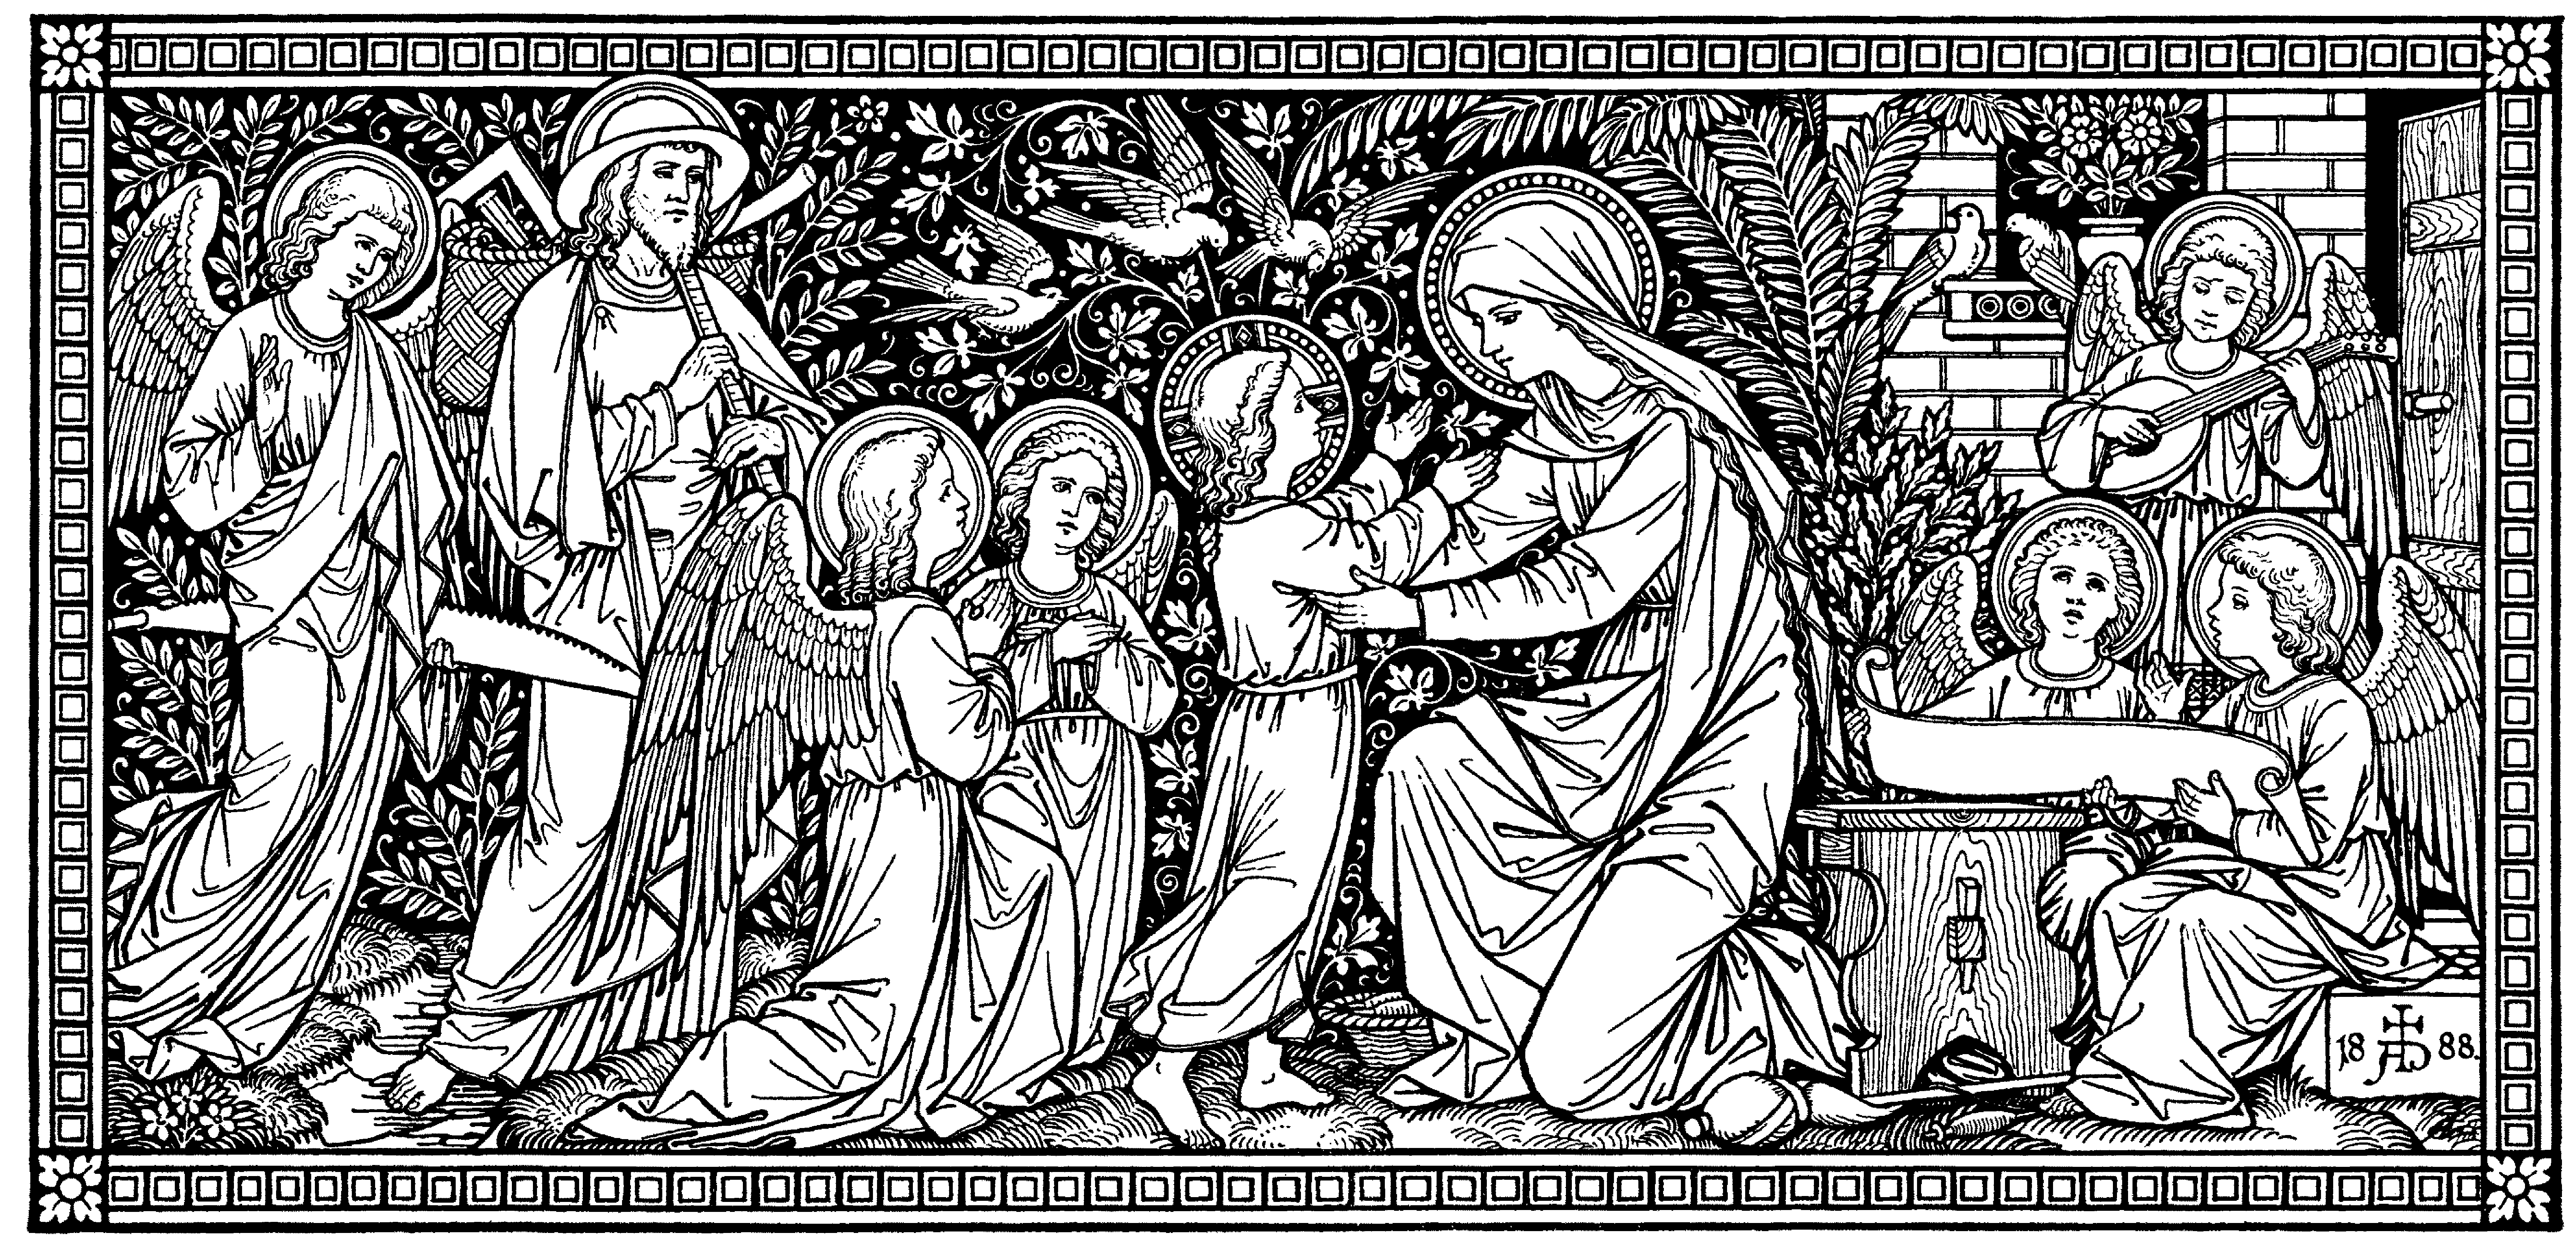
\includegraphics[height=5.5cm]{images/SainteFamille}
%\end{center}





\end{document}